\documentclass[11pt]{beamer}
\usepackage[utf8]{inputenc}
\usepackage[T1]{fontenc}
\usepackage{lmodern}
\usepackage[english]{babel}
\usepackage{amsmath}
\usepackage{amsfonts}
\usepackage{amssymb}
\usepackage{graphicx}
\usetheme{Warsaw}

\newcommand{\norm}[1]{\left\lVert#1\right\rVert}
\newcommand{\normsq}[1]{\left\lVert#1\right\rVert^2}


\newcommand{\MX}{\mathbf{X}} %uncentered data
\newcommand{\MC}{\mathbf{C}} %centering
\newcommand{\MY}{\mathbf{Y}} %centered data
\newcommand{\MF}{\mathbf{F}_2} %F2-distance matrix
\newcommand{\MFT}{\mathbf{F}_3} %F3-distance matrix
\newcommand{\MP}{\mathbf{P}} % PCs
\newcommand{\ML}{\mathbf{L}} % loadings
\newcommand{\MK}{\mathbf{K}} % Kernel
\newcommand{\MSINGULAR}{\mathbf{\Sigma}} % Singular values matrix
\newcommand{\MEIGEN}{\mathbf{\Lambda}} % Eigenvalue matrix


\newcommand{\MEAN}{\boldsymbol{\mu}} % Kernel


\begin{document}
	%\author{}
	%\title{}
	%\subtitle{}
	%\logo{}
	%\institute{}
	%\date{}
	%\subject{}
	%\setbeamercovered{transparent}
	%\setbeamertemplate{navigation symbols}{}
	\begin{frame}[plain]
		\maketitle
	\end{frame}
	
	\begin{frame}
		\frametitle{Principal Component Analysis}
		\begin{columns}
		\begin{column}{0.5\textwidth}
		\includegraphics<1>{figures/pca1.pdf}
		\includegraphics<2>{figures/pca2.pdf}
		\includegraphics<3>{figures/pca3.pdf}
		\includegraphics<4>{figures/pca4.pdf}
		\includegraphics<5>{figures/pca5.pdf}						
		\includegraphics<6>{figures/pca6.pdf}								
		\end{column}
		\begin{column}{0.5\textwidth}
		\begin{itemize}
		\item<1-> Raw SNP data $\MX; x_{ij}$
		\item<2-> Centering $\MY = \MC\MX; y_{ij}= x_{ij} - \mu_j$
		\only<3>{\item<3> Rotation $\MY = \underbrace{\MP}_\text{PCs}\underbrace{\ML}_\text{Rotation}$}
		\item<4-> Rotation $\MY = \MP\ML$		
		\item<5-> Truncation $\hat{\MP} = \begin{pmatrix}
		\mathbf{p}_1\\
		\mathbf{p}_2\\		
		\hline\\
		\vdots\\
		\mathbf{p}_n\\		
		\end{pmatrix} $		
		\item<6-> Approximation $\hat{\MY} = \hat{\MP}\hat{\ML}		$
		
		\end{itemize}
		
		\end{column}
		\end{columns}
	\end{frame}



\begin{frame}
	\frametitle{How to find PCs}
\begin{columns}
	\begin{column}{0.4\textwidth}
	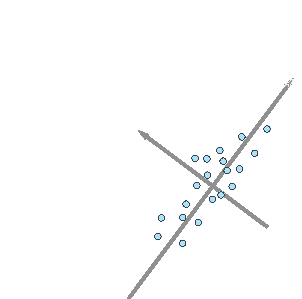
\includegraphics[width=\textwidth]{figures/pca3.pdf}
	\end{column}
	\begin{column}{0.6\textwidth}
	\begin{itemize}
	\item<1-> Singular Value Decomposition: $\MY = (\mathbf{U}\mathbf{D})\mathbf{L} = \mathbf{P}\mathbf{L}$
	\item<2-> Eigendecomposition of $\MY\MY^T$: $\MY\MY^T = \mathbf{U}\mathbf{D}^2\mathbf{U}^T = \MP\MP^T$
	\only<3>{\item $y_{ij}$}
	\item<4-> $y_{ij} = \sum_l (x_{il} - \mu_l)(x_{jl} - \mu_l)$
	\item<5-> $y_{ij} = F_3(\MEAN; \MX_i, \MX_j)$
	\end{itemize}
	\end{column}			
\end{columns}
\vspace{30px}
\only<6>{
\begin{alertblock}{Observation}
PCA is equivalent to outgroup-$F_3$-analysis with sample mean as outgroup
\end{alertblock}
}
\end{frame}


\begin{frame}
\frametitle{(metric) Multi-Dimensional Scaling (MDS)}

\begin{columns}
\begin{column}{0.5\textwidth}
\includegraphics<1>{figures/pca1.pdf}
\includegraphics<2>{figures/mds1.pdf}
\includegraphics<3->{figures/mds2.pdf}
\end{column}
\begin{column}{0.5\textwidth}
\includegraphics<4>{figures/mds3.pdf}		
\includegraphics<5>{figures/mds4.pdf}		
\includegraphics<6>{figures/mds5.pdf}		
\includegraphics<7>{figures/mds6.pdf}					
\end{column}
\end{columns}
\end{frame}


\begin{frame}
	\frametitle{PCA is MDS on $\MF$}
	
	\begin{itemize}
		\item<1-> PCA is decomposition of Covariance matrix: $\MY\MY^T$
		\item<2-> Consider $\MF; f_{ij} = F_2(X_i, X_j) = X_i^2 + X_j^2 - 2 X_i X_j$
		\item<3-> MDS is Eigendecomposition of $-\frac{1}{2}\MC\MF\MC$
		\item<4-> $\MC\MF\MC = \underbrace{\MC\MX_i^2\MC}_{0}  + \underbrace{\MC\MX_i^2\MC}_{0} - 2\underbrace{\MC\MX\MX^T\MC}_{\MY\MY^T}$
	\end{itemize}
	
	
	\only<5>{
		\begin{alertblock}{Observation}
			PCA is equivalent to MDS on $\MF$
		\end{alertblock}
	}
\end{frame}

\begin{frame}
	\frametitle{PCA is MDS on Outgroup$\MFT$}
	
	\begin{itemize}
		\item<1-> PCA is decomposition of Covariance matrix: $\MY\MY^T$
		\item<2-> Consider $\MFT(O); f_{ij} = F_3(O; X_i, X_j) = O^2 - OX_i - OX_j +  X_i X_j$
		\item<4-> $\MC\MFT\MC = \underbrace{\MC O^2\MC}_{0}  - 
		\underbrace{\MC O\MX_i\MC}_{0} -
		\underbrace{\MC O\MX_j\MC}_{0} + 
		\underbrace{\MC\MX\MX^T\MC}_{\MY\MY^T}$
	\end{itemize}
	
	
	\only<5>{
		\begin{alertblock}{Observation}
			Decomposition of \emph{any} centered $F_3$-matrix is equivalent to PCA.
		\end{alertblock}
	}
\end{frame}


\begin{frame}
\frametitle{0-diagonal MDS}
\end{frame}
	
\end{document}